\documentclass[12pt,journal,compsoc]{IEEEtran}
\usepackage{graphicx}

\newcommand\MYhyperrefoptions{bookmarks=true,bookmarksnumbered=true,
pdfpagemode={UseOutlines},plainpages=false,pdfpagelabels=true,
colorlinks=true,linkcolor={black},citecolor={black},pagecolor={black},
urlcolor={black},
pdftitle={Orbit Determination of 1951 Lick},
pdfsubject={Orbit Determination},
pdfauthor={Fengning Ding, Jason Liu, Patrick Rall},
pdfkeywords={Summer Science Program, 1951 Lick, Orbit Determination}}

%David: Let's follow some LaTex etiquette and put
%different sentences, phrases, large chunks, whatever in separate lines.
%Then, on git-hub, we would know precisely which sentence has changed.

\begin{document}

\title{Orbit Determination of 1951 Lick}

\author{Fengning~Ding,~Jason~Liu,~Patrick~Rall \\Summer Science Program 2011 at Westmont College}%
% Jason: I'm not sure if it's necessary to put "Summer Science Program Westmont 2011" here (or down below).
\markboth{Orbit Determination of 1951 Lick}{}

\IEEEcompsoctitleabstractindextext{%
\begin{abstract}
\boldmath
%David: The main point of our project is not to observe an asteroid, but to calculate its orbit. Accordingly, the 
%first letter of the abstract should be accordingly phrased.
During the summer of 2011, 
the asteroid 1951 Lick was observed on seven days using a 14'' Meade telescope and the 24'' Keck Telescope at Westmont College.
From seventeen usable images, the right ascension and declination of the asteroid were measured using least-squares plate reductions. 
Because the asteroid had just completed a retrograde loop at the time of observation, the rate of change of the range vector was small and difficult to compute.  
Existing well-developed orbital determination methods such as Gauss-Gibbs's method and Laplace's method are very sensitive to this rate of change, 
and both methods failed to give accurate orbital parameters. 
By using Laplace's method to first give reasonably correct estimates and then using five iterations of differential corrections to refine the preliminary results, it was possible to compute the orbit of the asteroid. 
While for most situations one iteration of differential corrections is enough, the inaccuracy of the initial estimate required multiple iterations to compensate.
This method produced spectacular results; 
relative to an observation made on July 19, the ephemeris calculated from the orbital elements determined was within 0.112 seconds of the right ascension and 1.56 arcseconds of the declination of the observed coordinates of the asteroid.  
The orbital elements from this analysis were consistent with previously determined measurements. 
This research demonstrates the possibility of computing orbits even in adverse situations and allows the usage of previously unusable data to furnish excellent orbital parameters.

\end{abstract}
}

%and a 20.5 x 16.4 mm CCD Camera (1280 x 1024 pixels)

\maketitle

\IEEEdisplaynotcompsoctitleabstractindextext
\IEEEpeerreviewmaketitle

\section{Introduction}
\IEEEPARstart{D}{ue}
to the potential of some near-Earth asteroids to collide with Earth, 
astronomers are especially interested in the orbits of near-Earth asteroids.
To ensure accurate monitoring of these hazardous objects, 
which often move in chaotic orbits perturbed by other planets, 
astronomers need to repeatedly measure the position and velocity with high precision to determine the orbit of the asteroid,
which is characterized by six parameters
corresponding to the six degrees of freedom of the initial conditions: %David: Do you like this tidbit? it can be deleted if you guys object
%Pato: yes, I do. Showing off is always good.
the semimajor axis $a$, 
the eccentricity $e$, 
the inclination with respect to the plane of the Earth's orbit $i$, 
the longitude of the ascending node with respect to the vernal equinox $\Omega$, 
the argument of the perihelion $\omega$, 
and the time of the last perihelion passage $T_p$.  
These orbital parameters can be used to locate the asteroid in the sky or to generate the position of the asteroid in the future.

In July 2011, as part of the Summer Science Program at Westmont College, the orbit of the asteroid 1951 Lick was determined. 
A 14''~telescope and the 24''~Keck Telescope at Westmont College were used to take seventeen images on seven different nights 
to determine the asteroid's right ascension $\alpha$ and declination $\delta$ at specific times.
The dataset of seventeen images is augmented by data collected by another team observing 1951 Lick consisting of Jeremy Hyde, Pathik Shah and Ming Zhao.
%Jason: Do we even need to include this line?
%Pato: Yes, we do.

Because the asteroid was leaving a retrograde loop, 
the equatorial unit vector $\hat{\rho}$ from the Earth to the asteroid changed very slowly, 
causing the classical Gauss-Gibbs orbit determination method, which is sensitive to $\frac{d\hat{\rho}}{dt}$, to give nonsensical values.
Laplace's method, 
another classical method of orbit determination, 
also initially gave inaccurate results.  
However, since the orbital parameters calculated from Laplace's method were at least very approximately correct, 
five iterations of differential corrections gave accurate orbital elements for the asteroid.
From the computed orbital elements, which are consistent with previous results, it was possible to accurately reproduce the ephemeris.

One novel aspect of this work is the application of five iterations of differential corrections. 
To determine the orbit from most sets
of observations, only one iteration was required to refine the results of either Gauss-Gibbs's method or Laplace's method.
However, because of the adverse positions of the Earth and the asteroid in their orbits, Laplace's method
gave only a very approximate estimate, so one differential correction did not give accurate orbital elements.
It was found that repeated iterations of differential corrections gave a series of orbital parameters that converged
to an accurate value. This extended orbital determination method could allow future astronomers to
compute orbits of objects in similarly unfavorable circumstances.

\section{Methods}
The images used for orbit determination were taken using two telescopes.
%Which ones?
After median-combining these images into series to reduce noise, 
a least-squares plate reduction (LSPR) was calculated
using star coordinate data from the Naval Observatory Merged Astrometric Dataset (NOMAD) database. 
These reductions yielded the right ascension $\alpha$ and declination $\delta$ for the asteroid at the observation times.
The orbital elements were determined using an implementation of Laplace's method of orbit determination with five iterations of differential corrections.

\subsection{Observing and Image Processing}
The asteroid was observed on seven days: July~1, July~3, July~8, July~10, July~16, July~19, and July~25, 2011 at 04:00-06:00 UTC.
%\footnote{All times are given in Universal Coordinated Time (UTC) unless otherwise specified.} each day.
%Footnote not needed since we only mention time once.
First, 
the approximate apparent $\alpha$ and $\delta$ of the asteroid was obtained from NASA's Jet Propulsion Laboratory's HORIZONS (JPL HORIZONS) ephemeris computation service.
TheSkyX software by Software Bisque was used to generate a star chart of the region of the sky in which the asteroid would be located.
After synchronizing and focusing the telescope on a nearby star, three or four series of five or seven images were taken with an exposure time of 45 seconds per image. For details see Table~\ref{tab:serieslist}.

When retrieving the approximate $\alpha$ and $\delta$ from JPL HORIZONS, 
data was collected for the apparent $\alpha$ and $\delta$, which compensated for various systematic errors such as atmospheric distortion.
However, the telescope already corrects for these effects, and so the asteroid was always located near the edge of the image. 
This error was discovered on July 19, and was eliminated in subsquent observations.

To remove noise and `hot pixels' (pixels that had been overexposed by a cosmic ray), 
the images for each series were flat-field corrected, manually aligned, and median combined 
using the MaxIm DL software by Diffraction Limited to form three processed images per observation.
The asteroid was identified on the three processed images of each observation 
by aligning and `blinking' (changing images over a short time period) the three images.
For an example of a processed image see Fig.~\ref{fig:exampleseries}.

\begin{figure}[!t]
\centering
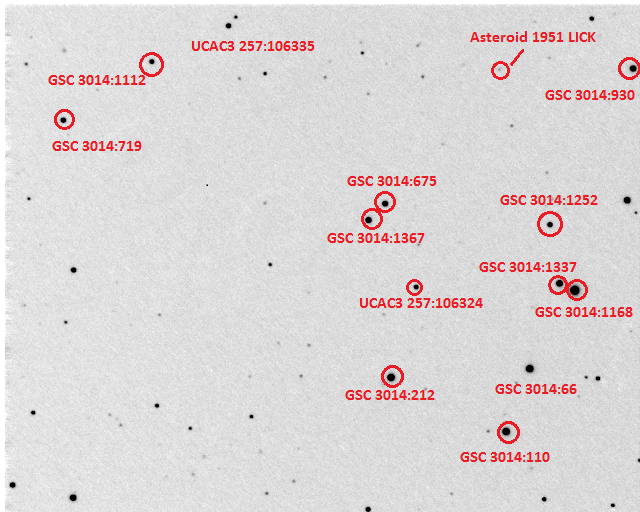
\includegraphics[width=3.4in]{Jul10Series2.png}
\caption{An example of a combined series of images: Series 2 of the observation on July 10 using the Meade 14'' telescope.\label{fig:exampleseries}}
\label{fig_sim}
\end{figure}

\begin{table}[!t]
\centering
\begin{tabular}{|c|c|c|c|c|}
\hline
Date & Telescope & Sync Star & Filter & \# images \\ \hline \hline
July 1 &Meade 14''& \multicolumn{3}{c|}{Omitted due to bad quality}\\ \hline \hline
July 3 & Keck 24''& Arcturis & Clear & 5 \\ \cline{4-5}
 & & & Clear & 5\\ \cline{3-5}
 & & \multicolumn{3}{c|}{Omitted due to bad quality} \\ \hline \hline
July 8 & Meade 14'' &\multicolumn{3}{c|}{Images are of wrong part of sky} \\ \cline{3-5}
 & & Phecda & Clear & 7 \\ \cline{4-5}
 & & & Clear & 7\\ \cline{4-5}
 & & & Clear & 7\\ \hline \hline
July 10 & Meade 14''& Phecda & Clear &7 \\ \cline{4-5}
 & & & Clear & 7\\ \cline{4-5}
 & & & Clear & 7\\ \hline \hline
July 16 & Meade 14''& Phecda & V-filter &5 \\ \cline{4-5}
 & & & Clear & 5\\ \cline{4-5}
 & & & Clear & 5\\ \cline{4-5}
 & & & Clear & 5\\ \cline{4-5}
 & & & Clear & 5\\ \hline \hline
July 19 & Meade 14''& Phecda & Clear &7 \\ \cline{4-5}
 & & & Clear & 7\\ \cline{4-5}
 & & & Clear & 7\\ \cline{4-5}
 & & & Clear & 7\\ \hline \hline
July 25 & Meade 14'' & Phecda & Clear &5 \\ \cline{4-5}
 & & & V-filter & 1\\ \hline
\end{tabular}
\caption{List of image series taken in observations of 1951 Lick in 2011\label{tab:serieslist}}
\end{table}

\subsection{Least-Squares Plate Reduction}
Using a Python program written by the authors, the LSPR was calculated for each processed image.
The centroids of numerous bright reference stars were obtained using MaxIm DL and compiled in a document along with the $\alpha$ and $\delta$ of the stars as given by NOMAD.
LSPR is a process to find the mapping between the plate $xy$ coordinates and the equatorial $\alpha\delta$ coordinates
that minimizes the least-squares residual. 
Before LSPR was performed, the effect of different angles of refraction for stars with higher and lower altitude was accounted for. 
By using the time of observation given by the FITS header of each image and taking into account the difference between the observatory's clock and the US Naval Observatory's clock, 
the local sidereal time was calculated to convert the equatorial coordinates from NOMAD of each reference star 
into theoretical values for local coordinates of altitude and azimuth.
Assuming an index of refraction of $n-1=58.2''$ for the atmosphere, the computed altitude of each star was adjusted to account for the resulting offset.
%Pato: Where is this angular estimate from? Cite!
The adjusted altitude and azimuth were then converted back to theoretical apparent equatorial coordinates.

To find the mapping between the plate $xy$ coordinates and the equatorial $\alpha\delta$ coordinates by LSPR, a least-squares linear fit that mapped the $xy$ plate coordinates of each star to its theoretical apparent equatorial coordinates was computed.
Using this mapping, the apparent equatorial coordinates of the center of the image were obtained to calculate the standard $\xi\eta$ coordinates for each reference star.\footnote{See [2]} Because the standard coordinates are truly linear functions of the plate coordinates, a more accurate least-squares fit was computed that maps the plate coordinates to the standard coordinates.
Using this linear transformation, the $\xi\eta$ coordinates of the asteroid were obtained, from which the apparent $\alpha$ and $\delta$ of the asteroid were calculated.
Finally, the apparent equatorial coordinates were transformed back to equatorial coordinates using the same index of refraction of the atmosphere.

To obtain an estimate of the uncertainty of the $\alpha$ and $\delta$ of the asteroid, the deviation of the predicted equatorial coordinates of each star and the catalogued coordinates were computed assuming two degrees of freedom.
This residual was possibly due to defects in the CCD chip and telescope mirror, aberration of starlight, inaccurate tabulations of reference star coordinates, or uncertainties in the centroid computations.

\subsection{Orbit Determination using Laplace's Method}
From the measured $\alpha$ and $\delta$ of the asteroid, the classical orbital elements of the asteroid were determined. 
Because the asteroid had recently exited from a retrograde loop,
the asteroid's position relative to Earth as a function of time was approximately a straight line,
resulting in small values for the change in velocity of the unit range vector $\hat{\rho}$, $\frac{d^2\hat{\rho}}{d\tau^2}$.\footnote{$\tau$ is the modified time given by $\tau=kt$, for ordinary time $t$ and the Gaussian gravitation constant $k=0.017...$.
All time derivatives in this section are with respect to modified time.}
The Gauss-Gibbs method of orbit determination\footnote{Described in [1]}, which is
sensitive to values of $\frac{d^2\hat{\rho}}{d\tau^2}$, produced unrealistic results, and so Laplace's method was used.

Five observations were used to obtain $\frac{d\hat{\rho}}{d\tau}$ and $\frac{d^2\hat{\rho}}{d\tau^2}$ for the middle observation.
The five unit equatorial vectors are given by $\hat{\rho}_1$, $\hat{\rho}_2$, $\hat{\rho}_3$, $\hat{\rho}_4$ and $\hat{\rho}_5$. The middle range vectors give the position of the asteroid on July 8 and were used to accurately estimate $\frac{d\hat{\rho}}{d\tau}$.
The second derivative of $\hat{\rho}$ at the middle observation was approximated using $\hat{\rho}_1$, $\hat{\rho}_3$, and $\hat{\rho}_5$, 
the range vectors of the asteroid on June 27, July 8, and July 25 respectively\footnote{The June 27 data was obtained by the other team with Jeremy Hyde, Pathik Shah, and Ming Zhao.}.
This time span was chosen to be large enough for the first derivative to change appreciably.

%Jason: Is this footnote necessary? (about The June 27 data was obtained by the other team)

To compute the first derivative, a second-order Taylor expansion was used:
\begin{eqnarray*}
\hat{\rho}_4&=&\hat{\rho}_3+\hat{\rho}_3' (\tau_4-\tau_3)+\frac{1}{2}\hat{\rho}_3'' (\tau_4-\tau_3)^2\\
\hat{\rho}_2&=&\hat{\rho}_3+\hat{\rho}_3' (\tau_2-\tau_3)+\frac{1}{2}\hat{\rho}_3'' (\tau_2-\tau_3) ^2\\
\end{eqnarray*}
which was solved for $\hat{\rho_3}'$.
The second derivative was calculated similarly but with $\hat{\rho}_1$ and $\hat{\rho}_5$ instead of $\hat{\rho}_2$ and $\hat{\rho}_4$.
From $\frac{d\hat{\rho}}{d\tau}$ and $\frac{d^2\hat{\rho}}{d\tau^2}$, the standard Laplace method was used to generate the position and velocity vectors of the asteroid\footnote{See [1]}.
This calculation was done using a script written in Python.

From the preliminary position and velocity, an ephemeris was generated for the times of each of the observations, and the differences from the measured values $\Delta \alpha$ and $\Delta \delta$ were calculated.
A small change in the position and velocity results in changes of $\alpha$ and $\delta$ according to the equations below:
\begin{eqnarray*}
\Delta \alpha &=& \frac{\partial \alpha}{\partial r_x} \Delta r_x + \frac{\partial \alpha}{\partial r_y} \Delta r_y + \frac{\partial \alpha}{\partial r_z} \Delta r_z + \\& &
\frac{\partial \alpha}{\partial v_x} \Delta v_x + \frac{\partial \alpha}{\partial v_y} \Delta v_y + \frac{\partial \alpha}{\partial v_z} \Delta v_z \\
\Delta \delta &=& \frac{\partial \delta}{\partial r_x} \Delta r_x + \frac{\partial \delta}{\partial r_y} \Delta r_y + \frac{\partial \delta}{\partial r_z} \Delta r_z + \\& &
\frac{\partial \delta}{\partial v_x} \Delta v_x + \frac{\partial \delta}{\partial v_y} \Delta v_y + \frac{\partial \delta}{\partial v_z} \Delta v_z
\end{eqnarray*}
Using six observations of the asteroid, least-squares corrections $\Delta r_x$, $\Delta r_y$, $\Delta r_z$, $\Delta v_x$, $\Delta v_y$, and $\Delta v_z$ for the position and velocity vectors were found.
Due to inaccurate preliminary vectors, these corrected positions and velocities were still not accurate since the differential corrections described above only correct for small inaccuracies, and so this process was iterated five times until the computed orbital elements converged. In each iteration, the last adjusted result for position and velocity was used to calculate new corrections according to the 
above procedure. As Table~\ref{tab:iterations} shows, Laplace's method gives inaccurate results for $\omega$ and $T_P$.
%Pato: I do not see how we can argue improvement of time of perihelion of the HORIZONS value is more wrong than our initial value.
With one iteration of corrections, $\omega$ and $T_P$ are much more accurate, but the other orbital elements
are over-corrected. Each subsequent iteration improves the value of all orbital elements.

\begin{table}[!t]
\centering
\begin{tabular}{|c|c|c|c|c|c|c|}
\hline
No. of Corrections & $a$ [AU]& $e$ & $i$ [$^\circ$] \\ \hline
Laplace's Method &1.376& 0.0699& 39.447 \\ \hline
One iteration &1.342& 0.0576& 38.968 \\ \hline
Two iterations &1.384& 0.0592& 39.078 \\ \hline
Three iterations &1.389& 0.0604& 39.087 \\ \hline
Four iterations &1.389& 0.0604& 39.088 \\ \hline
Five iterations &1.389& 0.0605& 39.088 \\ \hline
HORIZONS Value & 1.390536 & 0.0616082& 39.08962  \\ \hline \hline
No. of Corrections & $\Omega$ [$^\circ$] & $\omega$ [$^\circ$] & $T_P$ [JD]\\ \hline
Laplace's Method & 129.761& 344.711& 2455602.859\\ \hline
One iteration & 131.535& 163.598& 2455298.593\\ \hline
Two iterations & 130.852& 142.718& 2455243.991\\ \hline
Three iterations & 130.777& 140.797& 2455238.203\\ \hline
Four iterations & 130.773& 140.700& 2455237.901\\ \hline
Five iterations & 130.772& 140.695& 2455237.885\\ \hline 
HORIZONS Value & 130.769445 & 140.4418 & 2455835.571 \\ \hline
\end{tabular}
\caption{\label{tab:iterations} 1951 Lick orbital element outputs of Laplace's method, iterations of differential correction, and JPL HORIZONS.}
\end{table}

To compute the uncertainties for the orbital elements, a normal distribution according to the standard deviation computed from the LSPR for the $\alpha$ and $\delta$ of the asteroid was assumed.
A Monte-Carlo method with sample size of five hundred was used to compute the orbital elements using the procedure specified above for a set of asteroid coordinates randomly sampled from the Gaussian distribution.
The standard deviation of the computed orbital elements was reported as the uncertainty.

\subsection{Photometry}
On July 16 and July 25, 2011, a V-filter image of the asteroid was taken to measure the V-magnitude of the asteroid.
To determine the apparent magnitude of the asteroid, images were taken with a V-filter in the telescope, 
instead of the clear filter that was used for astrometry.
After taking a series of images with the V-filter, V-magnitudes of surrounding stars were obtained from the NOMAD database.
From the V-magnitudes of the reference stars, MaximDL computed the V-magnitude of the asteroid. See Table~\ref{tab:vmag}.

\begin{table}[!t]
\centering
\scalebox{0.9}{
\begin{tabular}{|c|c|c|}
\hline
Asteroid V-mag & Observation & Sync Star V-mag \\ \hline \hline
16.861 & GSC 2531:1730 & 12.690 \\ \hline
17.122 & GSC 2529:1728 & 12.590 \\ \hline
\end{tabular}
}
\caption{V-magnitude of 1951 Lick \label{tab:vmag}}
\end{table}

\section{Results}

The result of the orbit determination along with the uncertainty are shown in Table~\ref{tab:orbitalelements}.

\begin{table}[!t]
\centering
\scalebox{0.9}{
\begin{tabular}{|c|c|c|}
\hline
$a$ & $e$ & $i$ \\ \hline
$1.3894 \pm 0.0094$ AU & $0.06053 \pm 0.0024$ & $39.089 \pm 0.019 ^{\circ}$ \\ \hline \hline
$\Omega$ & $\omega$ & $T_P$ \\ \hline
$130.7706 \pm 0.1415 ^{\circ}$ & $140.65 \pm 3.71 ^{\circ}$ & $2455237.7 \pm 11.3$ JD \\ \hline
\end{tabular}
}
\caption{Measured orbital elements of 1951 Lick \label{tab:orbitalelements}}
\end{table}


It is noted that the orbit of the asteroid is similar in eccentricity to that of Mars with $e = 0.093$ \cite{bib:HORIZONS}, and the point of perihelion is hard to distinguish from other points, so the values for $\omega$ and $T_p$ are more difficult to determine than the other orbital elements.

% Jason: No idea what to do with this picture. It's slightly better than it was before, though.
\begin{figure}[!t]
\centering
\includegraphics[width=3.5in]{Lick_Orbit2.png}
\caption{Position of the asteroid relative to the Earth.  The blue loop is that of the Earth's orbit, and the black loop is that of the asteroid.  The positions of the Earth, going clockwise, are those of July 25, July 8, and June 26; the positions of the asteroid, going clockwise, are those of July 25, July 8, and June 26. }
\label{fig_sim}
\end{figure}

\begin{table}[!t]
\centering
\scalebox{0.9}{
\begin{tabular}{|c|c|c|c|}
\hline
Quantity & Measurement & HORIZONS Value & Difference \\ \hline
$a$ & $1.3894 \pm 0.0094$ AU & 1.390536 AU & 0.0011 AU \\ \hline
$e$ & $0.06053 \pm 0.0024$ & 0.0616082 & 0.0011 \\ \hline
$i$ & $39.089 \pm 0.019^{\circ}$ & 39.08962$^{\circ}$ & 0.001$^{\circ}$\\ \hline
$\Omega$ & $130.7706 \pm 0.1415 ^{\circ}$ & 130.769445$^{\circ}$ & 0.0012$^{\circ}$\\ \hline
$\omega$ & $140.65 \pm 3.71 ^{\circ}$ &140.4418$^{\circ}$ & 0.21$^{\circ}$\\ \hline
$T_P$ & $2455237.7 \pm 11.3$ JD & 2455835.571 JD & 2.1 JD \\ \hline
\end{tabular}
}
\caption{Measured orbital elements in comparison with JPL HORIZONS orbital elements of 1951 Lick}
\label{tab:HORIZONScomparison}
\end{table}

\begin{table}[!t]
\centering
\scalebox{0.9}{
\begin{tabular}{|c|c|c|c|}
\hline
Date & Observed $\alpha$ & HORIZONS $\alpha$ & Computed $\alpha$ \\
\cline{2-4} & Observed $\delta$ & HORIZONS $\delta$ & Computed $\delta$ \\ \hline \hline
Jul 19 & 12h 24m 7.855s & 12h 24m 3.18s & 12h 24m 7.667s \\
\cline{2-4} & 35$^{\circ}$ 5' 27.33'' & 35$^{\circ}$ 5' 32.0'' & 35$^{\circ}$ 5' 28.89'' \\ \hline
\end{tabular}
}
\caption{Comparison of JPL HORIZONS ephemeris of 1951 Lick and ephemeris from determined orbital elements with observation data\label{tab:observationcomparison}}
\end{table}

\section{Conclusion}
JPL HORIZONS provides values for the orbital elements, which serve as a good comparison to computed results.
The differences between the orbital elements that were determined in the experimental procedure and those given by JPL are shown in Table \ref{tab:HORIZONScomparison}.
The difference between the values is always significantly less than the statistical errors. There are no discrepancies between
computed orbital elements and that stored in the JPL HORIZONS database.
An ephemeris for July 19 generated from determined orbital elements was also calculated and compared to observations, as in Table \ref{tab:observationcomparison}.
Since orbital elements are constantly changing due to perturbations from planets,
it is irrelevant to compare computed orbital elements with the 
orbital elements from HORIZONS, because computations are made to best fit the observations and not the orbit at any
precise epoch.
However, the accuracy of this orbit determination is of theoretical interest, because 
it demonstrates that accurate orbits can be determined even if Gauss-Gibb's method fails to deliver anything reasonable and Laplace's method
gives orbital elements that are fairly off due to a non-ideal location of an asteroid with respect to the Earth.

%From the orbital elements, it is clear that there is very low probability the asteroid will hit the Earth in the near future.
%With such a low eccentricity, the asteroid is in a highly circular orbit, minimizing perturbations from other planets.
%Since gravitational acceleration is independent of mass, the stability of the asteroid's orbit is comparable to that of Mars in the short term.
%The successful computation of the orbit of 1951 Lick is an interesting case study, considering the non-ideal location of the asteroid with respect to the Earth.
%Future groups would benefit from our method of orbit determination.

\section*{Acknowledgments}

The authors would like to thank Dr. Michael Faison, Mr. Martin Mason, and Mary Masterman, Dougal Sutherland, Becky Raph, and Sean Mattingly for their help debugging Python scripts, assistance with observations, and teaching us the methodology used in this project.
The authors are grateful for the collaboration with the other team observing 1951 Lick, consisting of Jeremy Hyde, Pathik Shah and Ming Zhao.


\begin{thebibliography}{1}
\bibitem{bib:Danby}
Danby, J. M. A. (1962). \emph{Fundamentals of Celestial Mechanics} New York: Macmillan, 1962. 
%J.M.A.~Danby. \emph{Fundamentals of Celestial Mechanics}, 1st~ed.\hskip 1em plus
%  0.5em minus 0.4em\relax New York: Macmillan, 1962.
\bibitem{bib:Tatum}
Tatum, J. B. (2002). \emph{Celestial Mechanics} Obtained from M. Mason in 2011
%J.B.~Tatum. \emph{Celestial Mechanics}, 1st~ed., 2002\hskip 1em plus
%  0.5em minus 0.4em\relax
\bibitem{bib:HORIZONS}
NASA Jet Propulsion Laboratory HORIZONS System. Retrieved from http://ssd.jpl.nasa.gov/?horizons.
\end{thebibliography}

\end{document}